\section{Molmassen wichtiger Atome}

\begin{tabular}{c | c | c }
\textbf{Symbol} & \textbf{Molekül} & \textbf{Molmasse} \\
\hline
\rule{0pt}{10pt} H & Wasserstoff & $1.008 \, \mathrm{\frac{g}{mol}}$ \\
\rule{0pt}{10pt} C & Kohlenstoff & $12.011 \, \mathrm{\frac{g}{mol}}$ \\
\rule{0pt}{10pt} N & Stickstoff & $14.007 \, \mathrm{\frac{g}{mol}}$ \\
\rule{0pt}{10pt} O & Sauerstoff & $15.999 \, \mathrm{\frac{g}{mol}}$ \\
\rule{0pt}{10pt} Al & Aluminium & $26.982 \, \mathrm{\frac{g}{mol}}$ \\
\rule{0pt}{10pt} Si & Silicium & $28.982 \, \mathrm{\frac{g}{mol}}$ \\
\end{tabular}

% \vfill\null
% \columnbreak



\section{Ansätze zu Dynamik-Aufgaben}

\subsection{Saugheber}
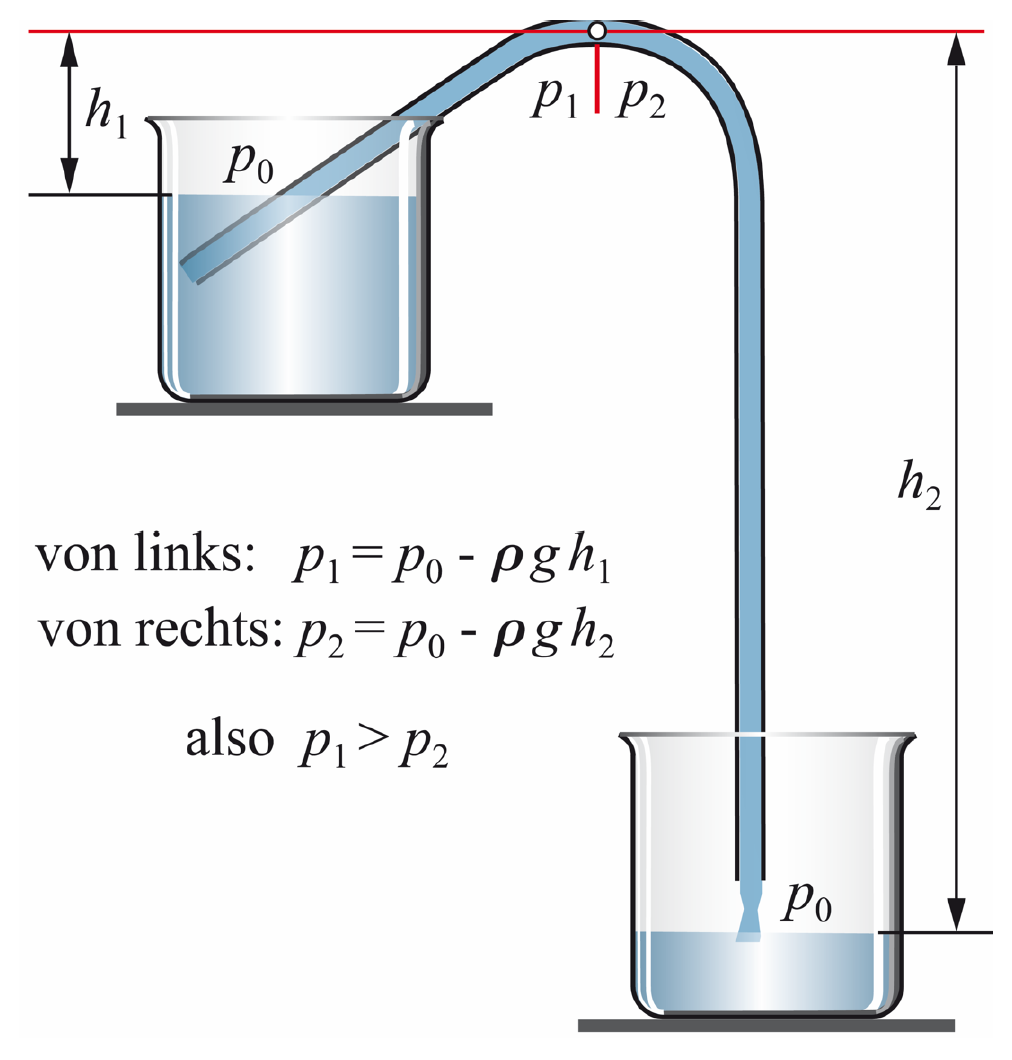
\includegraphics[width=.65\linewidth]{Bilder/saugheber.png}

\subsection{Barometer}
\begin{minipage}{0.4\linewidth}
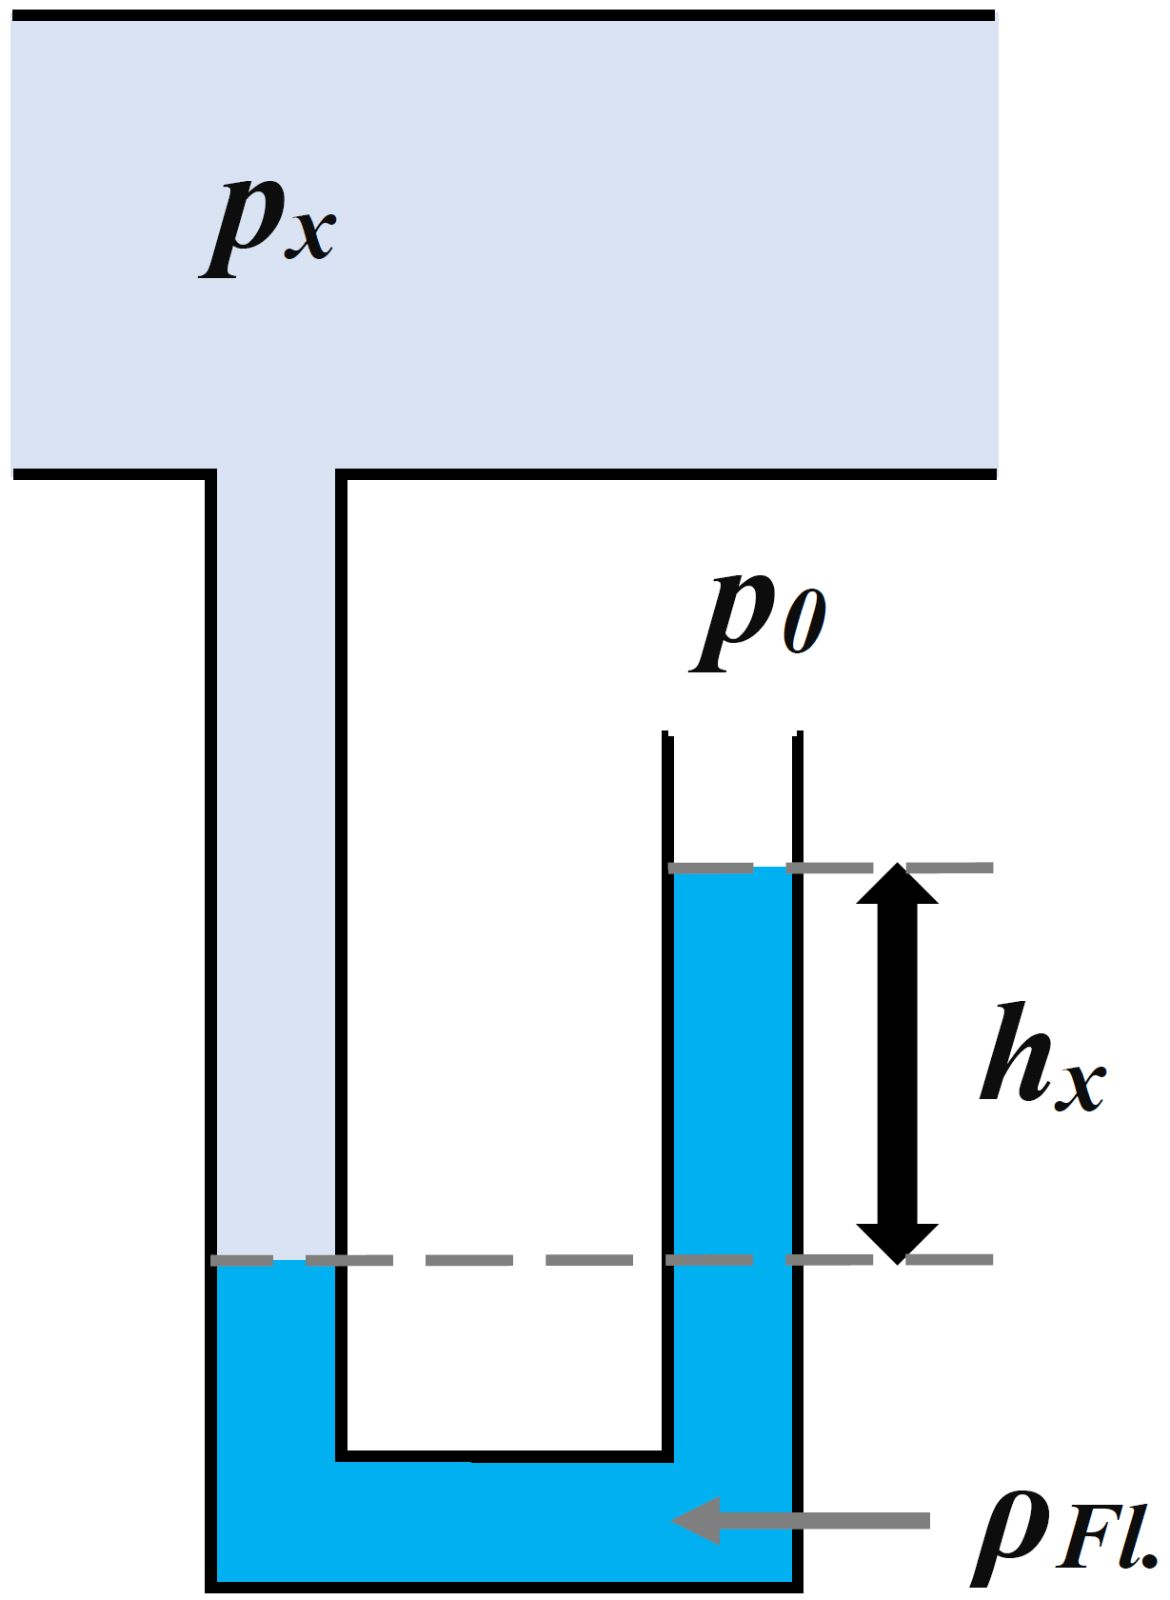
\includegraphics[width=\linewidth]{Bilder/manometer} \\
\end{minipage}
\hfill
\begin{minipage}{0.5\linewidth}
$\boxed{ p_x = p_0 + \underbrace{ \rho_{Fl} \cdot g \cdot h}_{\substack{p_s}} }$
 
 
\begin{tabular}{ll}
\\
$p_x$ & gemessener Druck \\
$p_0$ & Luftdruck \\
$p_s$ & Schweredruck \\
\\
\end{tabular}

$\Rightarrow$ Bernoulli \\
$\Rightarrow$ Kontinuität \\
\\
\\
\\
\\
\\
\end{minipage}




\subsection{Pitotrohr}
Prandtl'sches Staurohr; Staudruckmesser \\
Zur Messung von Strümungsgeschwindigkeiten \\
\\
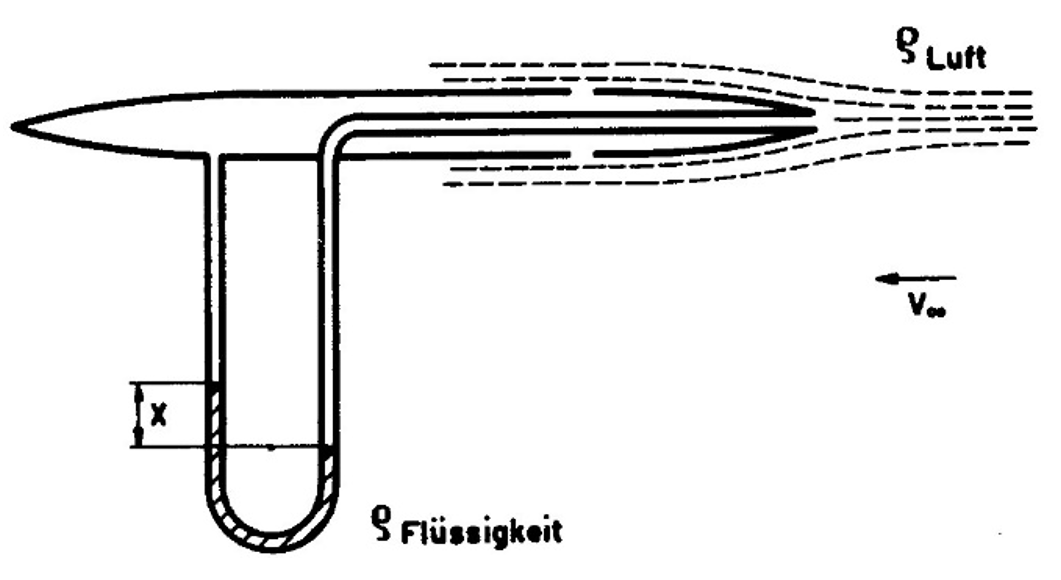
\includegraphics[width=0.7\linewidth]{Bilder/pitotrohr} \\

$$ \mathrm{Bernoulli \; horizontal:} \quad \boxed{  \underbrace{p_1}_{\substack{p_L}} + \frac{1}{2} \, \rho_1 \cdot \underbrace{v_1^2}_{\substack{0}} =  \underbrace{p_2}_{\substack{p_L - \Delta p}} + \frac{1}{2} \, \underbrace{\rho_2}_{\substack{\rho_L}} \cdot v_2^2} $$

$$ 0 = - \Delta p + \frac{1}{2} \, \rho_L \cdot v_2^2 \qquad \Rightarrow \Delta p =\frac{1}{2} \, \rho_L \cdot v_2^2 $$

$$ \mathrm{Gleichsetzen: } \quad \Delta p = \rho_{Fl} \cdot g \cdot h \quad \Rightarrow \quad v_2 = \sqrt{\frac{2 \cdot \rho_{Fl} \cdot g \cdot \Delta h}{\rho_L}} $$


\subsection{Venturirohr}
$$  \boxed{ Q = A_1 \sqrt{\frac{2 \Delta p}{\rho \left( \frac{A_1^2}{A_2^2} - 1\right)}}  \quad \quad [Q] = \frac{kg}{m^3} } $$


\subsection{Pumpe}
$$ \boxed{ W = P \cdot t = F \cdot \Delta s = p \cdot A \cdot \Delta s = p \cdot \Delta V }  $$

$$ \boxed{ P =  \frac{W}{t} = \frac{p \cdot V}{t} = p  \cdot  \dot{V} }  \quad  \boxed{ F = p \cdot A } $$



% \vfill\null
% \columnbreak


\subsection{Bewegungen}

$$ \boxed{ P = F \cdot v } \quad \boxed{ E_{kin} = \frac{1}{2} \, m \cdot v^2 } $$


\subsection{U-Rohr}

\begin{minipage}{0.4\linewidth}
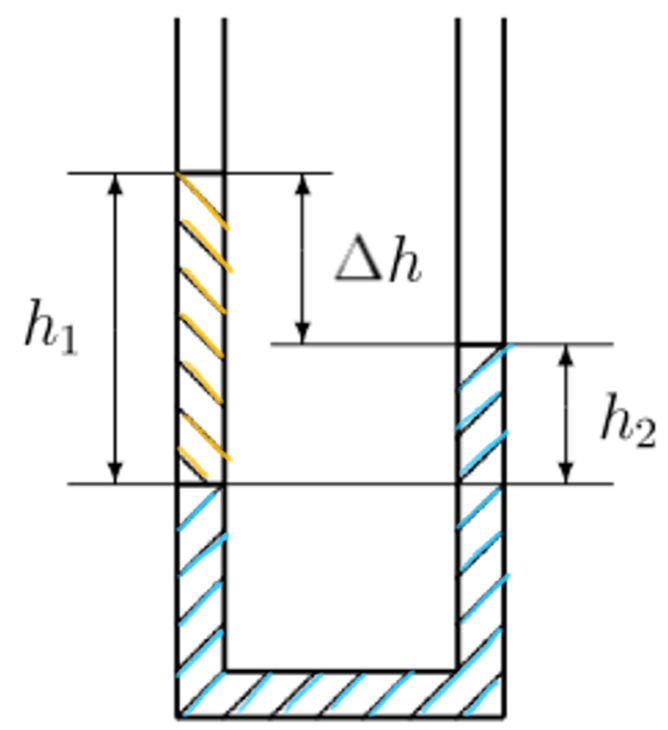
\includegraphics[width=\linewidth]{Bilder/u-rohr} \\
\end{minipage}
\hfill
\begin{minipage}{0.55\linewidth}
Ansatz: Druckgleichgewicht 

$$ p_1 = p_2 $$

$$ \rho_1 \cdot g \cdot h_1 = \rho_2 \cdot g \cdot h_2  $$
\end{minipage}


\subsection{Springbrunnen}

Ein Springbrunnen erzeugt einen $[x]$m hohen Wasserstrahl. Der Düsendurchmesser ist $[d_1]$, der Rohrdurchmesser zum Brunnen $[d_2]$, eine Pumpe für den Betrieb steht $[y]$m unterhalb des Brunnens. \\
Gesucht: Pumpdruck, Pumpenleistung bei $\eta$ = 90 $\%$\\
\\
$$\text{Bernoulli:} \quad  \overbrace{ p_1 + \frac{1}{2}\rho v_1^2}^{\text{Pumpe}} = \overbrace{p_2 + \frac{1}{2}\rho v_2^2 + \rho g y}^{\text{Düse}}, \quad v_1A_1 = v_2A_2 $$
$$ \frac{1}{2}mv^2_2 = mgx \Rightarrow v_2 = \sqrt{2gx}, \quad v_1 = v_2\frac{A_2}{A_1} = v_2\left(\frac{d_2}{d_1}\right)^2 $$
$$ \Delta p = p_1 - p_0 = \rho g y + \frac{1}{2}\rho v_2^2 - \frac{1}{2}\rho v_1^2 $$
$$ P_{ideal} = \Delta p \dot{V}, \quad P_{Pumpe} = \frac{\Delta p \dot{V}}{\eta} $$


\subsection{Wasser mit Dampf erhitzen}

Ein Tasse mit einer Masse $m_W$ Wasser und einer Temperatur von $T_K$ wird an
der Wasserdampfdüse einer Kaffeemaschine mittels Wasserdampf erhitzt. Der aus der
Kaffeemaschine ausströmende Wasserdampf ist $T_H$ heiss. Am Schluss haben sie 10 \%
mehr Wasser in der Tasse. (entspricht $m_D$)\\
Wie warm ist das Wasser nun? \\
\\
Ansatz: 1. Hauptsatz \quad $Q_{zu} = Q_{ab}$ \\
\\
$$ m_W \cdot c_W \, (T_M - T_K) = q_s \cdot m_D + m_D \cdot c_W \, (T_H - T_M) $$



\subsection{Eis in Wasser schmelzen}

In einem Gefäss befinden sich eine Masse $m_W$ Wasser. Dazu wird ein Eiswürfel mit Masse $m_E$ gegeben. Das Eis hat eine Temperatur $T_E$ und das Wasser hat eine Temperatur $T_W$. Die Temperatur $T_0$ steht für $0 \, \text{°C}$ bzw. 273.15 K \\
Gesucht ist die Mischtemperatur $T_M$ 

$$ \Delta Q_{ab} = \Delta Q_{zu}$$
$$ m_W \cdot c_W \cdot (T_W - T_M) = m_E \cdot \left( c_E \cdot (T_E - T_0) + q_f  +  c_W \cdot (T_M - T_0) \right) $$

\subsection{Beschlagenes Fenster}

Gesucht: Aussentemperatur $T_a$\\
Gegeben: Innentemperatur $T_i$, Luftfeuchtigkeit $f_i$ in $\%$, 
Wärmedurchgangszahl des Fensters $k$ und Wärmeübergangszahl $\alpha_i$\\

Beschlag bei $p_s(T_{fi}) = f \cdot p_s(T_i) \Rightarrow T_{fi} $ mittels Magnusformel bestimmen\\

Wärmestromdichte in allen Schichten gleich: $k(T_a - T_i) = \alpha_i(T_{fi} - T_i)$

\subsection{Luftbefeuchter}
Gesucht: rel. Luftfeuchtigkeit $f_{ri}$ \\
Gegeben: Volumen des Zimmers $V$, Menge verdampftes Wasser $m$, Zeit für kompletten Austausch $t$, Innentemperatur $T_i$, Aussentemperatur $T_a$, Luftfeuchtigkeit $f_{ra}$\\
$\dot{m}$ = Massenfluss (ai=nach innen, b=Befeuchter, ia=nach draussen)\\
$\dot{V} = \frac{V}{t} \quad [\frac{m^3}{s}] , \quad \quad \dot{m}_b = \frac{m}{t_0} \quad [\frac{kg}{s}], \quad \quad  M = \text{0.018} \frac{kg}{mol}$\\ 
$\rho_s = [\frac{kg}{m^3}]$ (Sättigungsdichte)

\begin{center}
    \begin{tabular}{c} 
    \\
    $ \dot{m}_{ai} + \dot{m}_b = \dot{m}_{ia} $ \\
    \\
    $ \dot{m} = f_r \cdot \rho_s \cdot \dot{V} $ \\
    \\
    $ f_{ra} \cdot \rho_{sa} \cdot \dot{V} + \dot{m}_b = f_{ri} \cdot \rho_{si} \cdot \dot{V} $ \\
    \\
    $ \rho_s = p_s (\theta) \cdot \frac{M}{R \cdot T_i} $ (Magnusformel für $p_s(T_a \text{resp.} T_i)$) \\
    \end{tabular}
\end{center}


